% questions.tex —— 2007 年·普通高等学校招生考试·四川卷·文科 · 题目内容片段（无答案）
% 由 tools/generate_projects.py 依来源总账自 2007/2007_数学真题_四川文_试题.md 生成，勿手改（改源 MD 后重跑）


状态：needs-review；依固定候选 PDF 两页（印刷页 411–412）三栏图像逐题核验，图形已矢量重绘，正式构建与逐页验收见回执。源未列各题分值，不补分值。第 12 题四选项与按题设计算的边长无一相符、第 21 题椭圆方程漏印等号、第 17 题题干有排印疑误，均照原页字面保留并登记问题。

\gkpart{一、选择题}

\begin{question}
\gkti{1}设集合 $M=\{4,5,6,8\}$，集合 $N=\{3,5,7,8\}$，那么 $M\cup N=$（　）

（A）$\{3,4,5,6,7,8\}$

（B）$\{5,8\}$

（C）$\{3,5,7,8\}$

（D）$\{4,5,6,8\}$

\Needspace{0.4\textheight}
\end{question}
\begin{question}
\gkti{2}函数 $f(x)=1+\log_2 x$ 与 $g(x)=2^{-x+1}$ 在同一直角坐标系下的图象大致是（　）
\nopagebreak[4]
\begin{center}% 2007 年四川卷文科第 2 题：四选项图象。
% 来源 PDF：普通高考/2007/2007四川文.pdf，SHA256 1318df44733ec939e8789379d6fa2115a2c6a63e84b73c1f2bf3c080007ce68c
% 原页：第 1 页（A3 三栏）第 1 栏，印刷页 411，图在题干下方。
% 重绘依据：四图 2×2 排列，(A) 递增曲线零点在 x=1、(B) 递减曲线 y 轴截距为 1、(C) 为正确图象（零点 1/2、截距 2、交点 (1,1)）、(D) 两曲线均递增；逐幅与文科原页比对一致。
\begin{tikzpicture}[scale=1.08, semithick, >=Stealth,
  every node/.style={inner sep=1.5pt}]
  % 四个等大的坐标系框（仅平移，画法完全一致）
  \foreach \dx/\dy/\opt in {0/0/A, 4.9/0/B, 0/-4.4/C, 4.9/-4.4/D}{
    \draw[->] ({\dx-0.65},\dy) -- ({\dx+2.85},\dy);
    \draw[->] (\dx,{\dy-0.7}) -- (\dx,{\dy+2.95});
    \node[anchor=north west] at ({\dx+1.07},{\dy-0.07}) {$1$};
    \node[anchor=north west] at ({\dx+2.07},{\dy-0.07}) {$2$};
    \node[anchor=east] at ({\dx-0.28},{\dy+1}) {$1$};
    \node[anchor=east] at ({\dx-0.28},{\dy+2}) {$2$};
    \node[anchor=north east] at ({\dx-0.08},{\dy-0.08}) {$O$};
    \node[anchor=west] at ({\dx+2.92},\dy) {$x$};
    \node[anchor=south west] at (\dx,{\dy+2.97}) {$y$};
    \node[anchor=east] at ({\dx-0.72},{\dy-0.56}) {(\opt)};
  }
  % (A) 递减过 (0,2)、递增过 (1,0)，交于 1<x<2
  \begin{scope}[shift={(0,0)}]
    \draw[domain=-0.35:2.45, samples=100, smooth]
      plot (\x,{2*exp(-0.65*\x)});
    \draw[domain=0.80:2.45, samples=100, smooth]
      plot (\x,{1.55*ln(\x)/ln(2)});
  \end{scope}
  % (B) 递减过 (0,1)、递增过 (0.5,0)，交于 x<1
  \begin{scope}[shift={(4.9,0)}]
    \draw[domain=-0.55:2.60, samples=100, smooth]
      plot (\x,{exp(-0.72*\x)});
    \draw[domain=0.42:2.15, samples=100, smooth]
      plot (\x,{ln(\x/0.5)/ln(2)});
  \end{scope}
  % (C) 真图象：f(x)=1+log_2 x 与 g(x)=2^{1-x}，交于 (1,1)
  \begin{scope}[shift={(0,-4.4)}]
    \draw[domain=-0.30:2.45, samples=100, smooth]
      plot (\x,{exp((1-\x)*ln(2))});
    \draw[domain=0.36:2.45, samples=100, smooth]
      plot (\x,{1+ln(\x)/ln(2)});
  \end{scope}
  % (D) 两条均递增，分别过 (-0.55,0)、(0.42,0)，交于 x≈1.3
  \begin{scope}[shift={(4.9,-4.4)}]
    \draw[domain=-0.64:2.50, samples=120, smooth]
      plot (\x,{1.35*ln(1+(\x+0.55)/1.1)});
    \draw[domain=0.18:1.90, samples=120, smooth]
      plot (\x,{1.60*sign(\x-0.42)*abs(\x-0.42)^1.25});
  \end{scope}
\end{tikzpicture}
\end{center}
\nopagebreak[4]
\end{question}
\begin{question}
\gkti{3}某商场买来一车苹果，从中随机抽取了 $10$ 个苹果，其重量（单位：克）分别为：$150$，$152$，$153$，$149$，$148$，$146$，$151$，$150$，$152$，$147$，由此估计这车苹果单个重量的期望值是（　）

（A）$150.2$ 克

（B）$149.8$ 克

（C）$149.4$ 克

（D）$147.8$ 克

\Needspace{0.4\textheight}
\end{question}
\begin{question}
\gkti{4}如图，$ABCD-A_1B_1C_1D_1$ 为正方体，下面结论错误的是（　）
\nopagebreak[4]
\begin{center}% 2007 年四川卷文科第 4 题：题图。
% 来源 PDF：普通高考/2007/2007四川文.pdf，SHA256 1318df44733ec939e8789379d6fa2115a2c6a63e84b73c1f2bf3c080007ce68c
% 原页：第 1 页（A3 三栏）第 1 栏，印刷页 411，图在题干下方。
% 重绘依据：斜投影正方体，A 左下、B 右下、A1 左上、B1 右上，D1 在 A1 右上方；可见棱实线、被遮棱与辅助线虚线；与文科原页逐线比对一致。
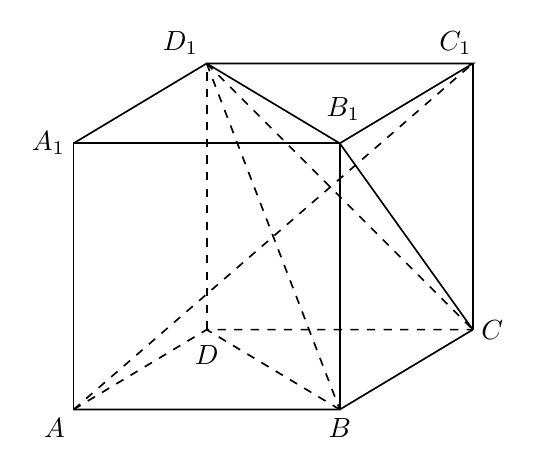
\begin{tikzpicture}[scale=1.3, semithick,
  every node/.style={inner sep=1.5pt}]
  \coordinate (A)  at (0,0);
  \coordinate (B)  at (2.6,0);
  \coordinate (A1) at (0,2.6);
  \coordinate (B1) at (2.6,2.6);
  \coordinate (D)  at (1.3,0.78);
  \coordinate (C)  at (3.9,0.78);
  \coordinate (D1) at (1.3,3.38);
  \coordinate (C1) at (3.9,3.38);
  % 不可见棱与不可见辅助线
  \draw[dashed] (A) -- (D) -- (C);
  \draw[dashed] (D) -- (D1);
  \draw[dashed] (B) -- (D);
  \draw[dashed] (D1) -- (B);
  \draw[dashed] (D1) -- (C);
  \draw[dashed] (A) -- (C1);
  % 可见棱
  \draw (A) -- (B) -- (C);
  \draw (A) -- (A1) -- (B1) -- (B);
  \draw (A1) -- (D1) -- (C1) -- (B1);
  \draw (C) -- (C1);
  % 可见辅助线
  \draw (B1) -- (D1);
  \draw (B1) -- (C);
  \node[anchor=north east] at ([xshift=-1pt,yshift=-1pt]A) {$A$};
  \node[anchor=north] at ([yshift=-1pt]B) {$B$};
  \node[anchor=west] at ([xshift=1pt]C) {$C$};
  \node[anchor=north] at ([yshift=-3pt]D) {$D$};
  \node[anchor=east] at ([xshift=-1pt]A1) {$A_1$};
  \node[anchor=south] at ([xshift=1pt,yshift=5pt]B1) {$B_1$};
  \node[anchor=south east] at ([xshift=1pt,yshift=1pt]C1) {$C_1$};
  \node[anchor=south east] at ([xshift=-1pt,yshift=1pt]D1) {$D_1$};
\end{tikzpicture}
\end{center}
\nopagebreak[4]
（A）$BD\parallel$ 平面 $CB_1D_1$

（B）$AC_1\perp BD$

（C）$AC_1\perp$ 平面 $CB_1D_1$

（D）异面直线 $AD$ 与 $CB_1$ 角为 $60^\circ$

\end{question}
\begin{question}
\gkti{5}如果双曲线 $\dfrac{x^2}{4}-\dfrac{y^2}{2}=1$ 上一点 $P$ 到双曲线右焦点的距离是 $2$，那么点 $P$ 到 $y$ 轴的距离是（　）

（A）$\dfrac{4\sqrt6}{3}$

（B）$\dfrac{2\sqrt6}{3}$

（C）$2\sqrt6$

（D）$2\sqrt3$

\Needspace{0.4\textheight}
\end{question}
\begin{question}
\gkti{6}设球 $O$ 的半径是 $1$，$A$、$B$、$C$ 是球面上三点，已知 $A$ 到 $B$、$C$ 两点的球面距离都是 $\dfrac{\pi}{2}$，且二面角 $B-OA-C$ 的大小为 $\dfrac{\pi}{3}$，则从 $A$ 点沿球面经 $B$、$C$ 两点再回到 $A$ 点的最短距离是（　）
\nopagebreak[4]
\begin{center}% 2007 年四川卷文科第 6 题：题图。
% 来源 PDF：普通高考/2007/2007四川文.pdf，SHA256 1318df44733ec939e8789379d6fa2115a2c6a63e84b73c1f2bf3c080007ce68c
% 原页：第 1 页（A3 三栏）第 2 栏，印刷页 411，图在题干下方。
% 重绘依据：圆表示球（半径 2），A 为上极点，赤道画成水平椭圆，B 在左、C 在右；O 到 A、B、C 的半径虚线；与文科原页比对一致。
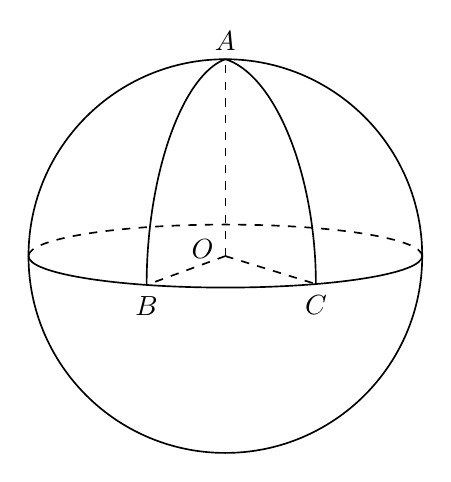
\begin{tikzpicture}[scale=1.25, semithick,
  every node/.style={inner sep=1.5pt}]
  % 球面轮廓与赤道
  \draw (0,0) circle (2);
  \draw[dashed] (2,0) arc[start angle=0, end angle=180, x radius=2, y radius=0.32];
  \draw (2,0) arc[start angle=0, end angle=-180, x radius=2, y radius=0.32];
  \coordinate (O) at (0,0);
  \coordinate (A) at (0,2);
  \coordinate (B) at (-0.800,-0.293);
  \coordinate (C) at (0.920,-0.284);
  % 球内半径（虚线）
  \draw[dashed] (O) -- (A);
  \draw[dashed] (O) -- (B);
  \draw[dashed] (O) -- (C);
  % 自 A 沿球面到 B、C 的经线弧（实线）
  \draw[domain=0:90, samples=80, smooth, variable=\t]
    plot ({2*sin(\t)*(-0.4000)},{2*cos(\t)+0.32*sin(\t)*(-0.9165)});
  \draw[domain=0:90, samples=80, smooth, variable=\t]
    plot ({2*sin(\t)*(0.4599)},{2*cos(\t)+0.32*sin(\t)*(-0.8881)});
  \node[anchor=south] at ([yshift=1pt]A) {$A$};
  \node[anchor=east] at ([xshift=-2pt,yshift=2pt]O) {$O$};
  \node[anchor=north] at ([yshift=-2pt]B) {$B$};
  \node[anchor=north] at ([yshift=-2pt]C) {$C$};
\end{tikzpicture}
\end{center}
\nopagebreak[4]
（A）$\dfrac{7\pi}{6}$

（B）$\dfrac{5\pi}{4}$

（C）$\dfrac{4\pi}{3}$

（D）$\dfrac{3\pi}{2}$

\end{question}
\begin{question}
\gkti{7}等差数列 $\{a_n\}$ 中，$a_1=1$，$a_3+a_5=14$，其前 $n$ 项和 $S_n=100$，则 $n=$（　）

（A）$9$

（B）$10$

（C）$11$

（D）$12$

\end{question}
\begin{question}
\gkti{8}设 $A(a,1)$、$B(2,b)$、$C(4,5)$ 为坐标平面上三点，$O$ 为坐标原点，若 $\overrightarrow{OA}$ 与 $\overrightarrow{OB}$ 在 $\overrightarrow{OC}$ 上的投影相同，则 $a$ 与 $b$ 满足的关系式为（　）

（A）$4a-5b=3$

（B）$5a-4b=3$

（C）$4a+5b=14$

（D）$5a+4b=14$

\end{question}
\begin{question}
\gkti{9}用数字 $1,2,3,4,5$ 可以组成没有重复数字，并且比 $20000$ 大的五位偶数共有（　）

（A）$48$ 个

（B）$36$ 个

（C）$24$ 个

（D）$18$ 个

\end{question}
\begin{question}
\gkti{10}已知抛物线 $y=-x^2+3$ 上存在关于直线 $x+y=0$ 对称的相异两点 $A$、$B$，则 $|AB|$ 等于（　）

（A）$3$

（B）$4$

（C）$3\sqrt2$

（D）$4\sqrt2$

\end{question}
\begin{question}
\gkti{11}某公司有 $60$ 万元资金，计划投资甲、乙两个项目，按要求对项目甲的投资不小于对项目乙投资的 $\dfrac23$ 倍，且对每个项目的投资不能低于 $5$ 万元，对项目甲每投资 $1$ 万元可获得 $0.4$ 万元的利润，对项目乙每投资 $1$ 万元可获得 $0.6$ 万元的利润，该公司正确规划投资后，在这两个项目上共可获得的最大利润为（　）

（A）$36$ 万元

（B）$31.2$ 万元

（C）$30.4$ 万元

（D）$24$ 万元

\Needspace{0.4\textheight}
\end{question}
\begin{question}
\gkti{12}如图，$l_1$、$l_2$、$l_3$ 是同一平面内的三条平行直线，$l_1$ 与 $l_2$ 间的距离是 $1$，$l_2$ 与 $l_3$ 间的距离是 $2$，正三角形 $ABC$ 的三顶点分别在 $l_1$、$l_2$、$l_3$ 上，则 $\triangle ABC$ 的边长是（　）
\nopagebreak[4]
\begin{center}% 2007 年四川卷文科第 12 题：题图。
% 来源 PDF：普通高考/2007/2007四川文.pdf，SHA256 1318df44733ec939e8789379d6fa2115a2c6a63e84b73c1f2bf3c080007ce68c
% 原页：第 1 页（A3 三栏）第 2 栏，印刷页 411，图在题干下方。
% 重绘依据：三条水平平行线自上而下 l1、l2、l3，间距按 1:2；A 在 l1 上居右，B 在 l2 上居左，C 在 l3 上；与文科原页比对一致。
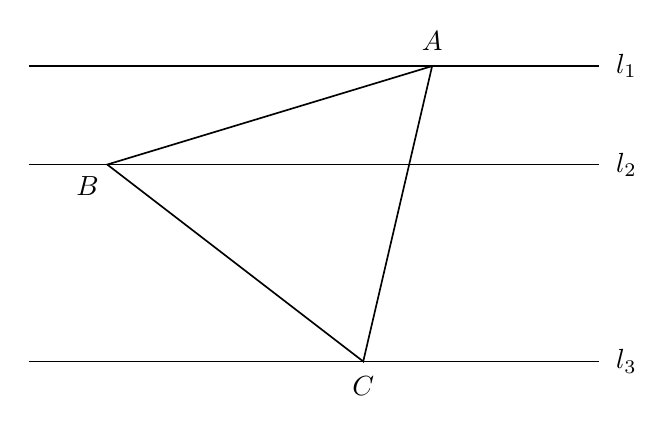
\begin{tikzpicture}[scale=1.25, semithick,
  every node/.style={inner sep=1.5pt}]
  % 三条平行线
  \draw (-0.2,2.2) -- (5.6,2.2);
  \draw (-0.2,1.2) -- (5.6,1.2);
  \draw (-0.2,-0.8) -- (5.6,-0.8);
  % 正三角形的三个顶点
  \coordinate (A) at (3.9,2.2);
  \coordinate (B) at (0.6,1.2);
  \coordinate (C) at (3.2,-0.8);
  \draw (A) -- (B) -- (C) -- cycle;
  \node[anchor=west] at (5.72,2.2) {$l_1$};
  \node[anchor=west] at (5.72,1.2) {$l_2$};
  \node[anchor=west] at (5.72,-0.8) {$l_3$};
  \node[anchor=south] at ([yshift=3pt]A) {$A$};
  \node[anchor=north east] at ([xshift=-1pt,yshift=-2pt]B) {$B$};
  \node[anchor=north] at ([yshift=-3pt]C) {$C$};
\end{tikzpicture}
\end{center}
\nopagebreak[4]
（A）$2\sqrt3$

（B）$\dfrac{4\sqrt6}{3}$

（C）$\dfrac{3-\sqrt7}{4}$

（D）$\dfrac{2-\sqrt{21}}{3}$

\end{question}
\gkpart{二、填空题}

\begin{question}
\gkti{13}$\left(x-\dfrac1x\right)^n$ 的展开式中的第 $5$ 项为常数项，那么正整数 $n$ 的值是\gkblank{}．

\Needspace{0.4\textheight}
\end{question}
\begin{question}
\gkti{14}如图，在正三棱柱 $ABC-A_1B_1C_1$ 中，侧棱长为 $\sqrt2$，底面三角形的边长为 $1$，则 $BC_1$ 与侧面 $ACC_1A_1$ 所成的角是\gkblank{}．
\nopagebreak[4]
\begin{center}% 2007 年四川卷文科第 14 题：题图。
% 来源 PDF：普通高考/2007/2007四川文.pdf，SHA256 1318df44733ec939e8789379d6fa2115a2c6a63e84b73c1f2bf3c080007ce68c
% 原页：第 1 页（A3 三栏）第 3 栏，印刷页 411，图在题干下方。
% 重绘依据：竖放正三棱柱斜二测画法，侧棱与底面边长之比按 √2:1；可见棱实线、不可见棱与 BC1 虚线；与文科原页比对一致。
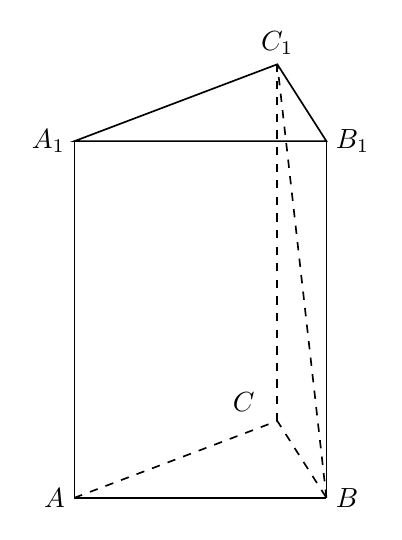
\begin{tikzpicture}[scale=1.6, semithick,
  every node/.style={inner sep=1.5pt}]
  \coordinate (A1) at (0,0);
  \coordinate (B1) at (2,0);
  \coordinate (C1) at (1.61,0.61);
  \coordinate (A)  at (0,-2.83);
  \coordinate (B)  at (2,-2.83);
  \coordinate (C)  at (1.61,-2.22);
  % 不可见的三条棱与辅助线
  \draw[dashed] (A) -- (C) -- (B);
  \draw[dashed] (C) -- (C1);
  \draw[dashed] (B) -- (C1);
  % 可见的侧棱与底边
  \draw (A1) -- (A);
  \draw (B1) -- (B);
  \draw (A) -- (B);
  % 上底
  \draw (A1) -- (B1) -- (C1) -- cycle;
  \node[anchor=east] at ([xshift=-1pt]A1) {$A_1$};
  \node[anchor=west] at ([xshift=1pt]B1) {$B_1$};
  \node[anchor=south] at ([yshift=1pt]C1) {$C_1$};
  \node[anchor=east] at ([xshift=-1pt]A) {$A$};
  \node[anchor=west] at ([xshift=1pt]B) {$B$};
  \node[anchor=south east] at ([xshift=-4pt,yshift=1pt]C) {$C$};
\end{tikzpicture}
\end{center}
\nopagebreak[4]
\end{question}
\begin{question}
\gkti{15}已知 $\odot O$ 的方程是 $x^2+y^2-2=0$，$\odot O'$ 的方程是 $x^2+y^2-8x+10=0$，由动点 $P$ 向 $\odot O$ 和 $\odot O'$ 所引的切线长相等，则动点 $P$ 的轨迹方程是\gkblank{}．

\end{question}
\begin{question}
\gkti{16}下面有五个命题：

① 函数 $y=\sin^4x-\cos^4x$，的最小正周期是 $\pi$；

② 终边在 $y$ 轴上的角的集合是 $\left\{\alpha\;\middle|\;\alpha=\dfrac{k\pi}{2},\;k\in\mathbf Z\right\}$；

③ 在同一坐标系中，函数 $y=\sin x$ 的图象和函数 $y=x$ 的图象有三个公共点；

④ 把函数 $y=3\sin\left(2x+\dfrac{\pi}{3}\right)$ 的图象向右平移 $\dfrac{\pi}{6}$ 得到 $y=3\sin2x$ 的图象；

⑤ 角 $\theta$ 为第一象限角的充要条件是 $\sin\theta>0$．

其中真命题的序号是\gkblank{}．（写出所有）

\end{question}
\gkpart{三、解答题}

\begin{question}
\gkti{17}厂家在产品出厂前，需对产品做检验，厂家对一般产品致冷商家的，商家符合规定拾取一定数量的产品做检验，以决定是否验收这些产品．

（1）若厂家库房中的每件产品合格的概率为 $0.3$，从中任意取出 $4$ 种进行检验，求至少要 $1$ 件是合格产品的概率；

（2）若厂家发给商家 $20$ 件产品，其中有 $3$ 件不合格，按合同规定该商家从中任取 $2$ 件，来进行检验，只有 $2$ 件产品合格时才接收这些产品，否则拒收，分别求出该商家计算出不合格产品为 $1$ 件和 $2$ 件的概率，并求该商家拒收这些产品的概率．

\end{question}
\begin{question}
\gkti{18}已知 $\cos\alpha=\dfrac17$，$\cos(\alpha-\beta)=\dfrac{13}{14}$，且 $0<\beta<\alpha<\dfrac{\pi}{2}$．

（1）求 $\tan2\alpha$ 的值；

（2）求 $\beta$．

\Needspace{0.4\textheight}
\end{question}
\begin{question}
\gkti{19}如图，$PCBM$ 是直角梯形，$\angle PCB=90^\circ$，$PM\parallel BC$，直线 $AM$ 与直线 $PC$ 所成的角为 $60^\circ$，又 $AC=1$，$BC=2PM=2$，$\angle ACB=90^\circ$．
\nopagebreak[4]
\begin{center}% 2007 年四川卷文科第 19 题：题图。
% 来源 PDF：普通高考/2007/2007四川文.pdf，SHA256 1318df44733ec939e8789379d6fa2115a2c6a63e84b73c1f2bf3c080007ce68c
% 原页：第 2 页（A3 三栏）第 1 栏，印刷页 412，图在题干下方。
% 重绘依据：P、M 在上方且 PM 水平，C 在 P 正下方，B 在 C 右侧，A 在左下方；可见线段实线，被梯形遮住的 PC、CB、AC 虚线，C 处画直角记号；与文科原页逐线比对一致。
\begin{tikzpicture}[scale=2.2, semithick,
  every node/.style={inner sep=1.5pt}]
  \coordinate (P) at (0,3);
  \coordinate (M) at (1,3);
  \coordinate (C) at (0,2);
  \coordinate (B) at (2,2);
  \coordinate (A) at (-0.95,1.55);
  % 被遮挡的三条线
  \draw[dashed] (P) -- (C);
  \draw[dashed] (C) -- (B);
  \draw[dashed] (A) -- (C);
  % 可见线段
  \draw (P) -- (M);
  \draw (P) -- (A);
  \draw (M) -- (B);
  \draw (A) -- (B);
  \draw (A) -- (M);
  % C 处直角记号
  \draw ($(C)+(0.18,0)$) -- ($(C)+(0.18,0.18)$) -- ($(C)+(0,0.18)$);
  \node[anchor=south east] at ([xshift=-1pt,yshift=1pt]P) {$P$};
  \node[anchor=south west] at ([xshift=1pt,yshift=1pt]M) {$M$};
  \node[anchor=north west] at ([xshift=2pt,yshift=-2pt]C) {$C$};
  \node[anchor=north west] at ([xshift=1pt,yshift=-1pt]B) {$B$};
  \node[anchor=north east] at ([xshift=-1pt,yshift=-1pt]A) {$A$};
\end{tikzpicture}
\end{center}
\nopagebreak[4]
（1）求证：$AC\perp BM$；

（2）求二面角 $M-AB-C$ 的大小；

（3）求多面体 $PMABC$ 的体积．

\end{question}
\begin{question}
\gkti{20}设函数 $f(x)=ax^3+bx+c$（$a\neq0$）为奇函数，其图象在点 $(1,f(1))$ 处的切线与直线 $x-6y-7=0$ 垂直，导函数 $f'(x)$ 的最小值为 $-12$．

（1）求 $a,b,c$ 的值；

（2）求函数 $f(x)$ 的单调递增区间，并求函数 $f(x)$ 在 $[-1,3]$ 上的最大值和最小值．

\end{question}
\begin{question}
\gkti{21}已知 $F_1$、$F_2$ 分别是椭圆 $\dfrac{x^2}{4}+y^2-1$ 的左、右焦点．

（1）若 $P$ 是第一象限内该椭圆上的一点，且 $\overrightarrow{PF_1}\cdot\overrightarrow{PF_2}=-\dfrac54$，求点 $P$ 的坐标；

（2）设过定点 $M(0,2)$ 的直线 $l$ 与椭圆交于不同的两点 $A$、$B$，且 $\angle AOB$ 为锐角（其中 $O$ 为作标原点），求直线 $l$ 的斜率 $k$ 的取值范围．

\end{question}
\begin{question}
\gkti{22}已知函数 $f(x)=x^2-4$，设曲线 $y=f(x)$ 在点 $(x_n,f(x_n))$ 处的切线与 $x$ 轴的交点为 $(x_{n+1},0)$（$n\in\mathbf N^*$），其中 $x_1$ 为正实数．

（1）用 $x_n$ 表示 $x_{n+1}$；

（2）若 $x_1=4$，记 $a_n=\lg\dfrac{x_n+2}{x_n-2}$，证明数列 $\{a_n\}$ 成等比数列，并求数列 $\{x_n\}$ 的通项公式；

（3）若 $x_1=4$，$b_n=x_n-2$，$T_n$ 是数列 $\{b_n\}$ 的前 $n$ 项和，证明 $T_n<3$．

\end{question}